\documentclass[12pt]{article}
\usepackage{amsmath}
\usepackage{csvsimple}
\usepackage{graphicx}
\graphicspath{ {./../images/} }
\usepackage{hyperref}
\usepackage[latin1]{inputenc}
\usepackage{listings}

\DeclareMathOperator{\Tr}{Tr}

\lstset{
  columns=fullflexible,
  breaklines=true,
}

\title{El Farol Bar Problem on a Social Network}
\author{Rebecca Cohen}

\begin{document}
\maketitle
\section{Abstract}
Does network structure determine which agents will attend the bar in a modified El Farol Bar problem.  In most cases, the network does not appear to converge to a single stable fixed point, but rather oscillates around an attractor in which some agents always attend and others attend in alternating weeks.  

\section{Introduction}
Motivate El Farol bar problem.  Work with social networks.

\section{Social Decision Function}
To test the hypothesis that local differences in the structure of social networks can encode the diversity of strategies required to regulate attendance, we construct a simple scenario in which each agent chooses to attend the bar if at least $\ell$ of the agent's neighbors attended the previous week.  We define the attendance vector $\vec{y}(t)$ such that
\begin{equation}
  y_i(t) = \begin{cases}
    1 &\text{if agent}\; i \; \text{attends on week t} \\
    0 &\text{otherwise}
  \end{cases}
\end{equation}

Then 
\begin{equation}
  \vec{y}(t + 1) = F(\mathbf{A}\vec{y}(t))
\end{equation}

where
\begin{equation}
  F(\vec{x})_i = \begin{cases}
    1 &\text{if} \; x_i > \ell \\
    0 &\text{otherwise}
  \end{cases}
\end{equation}

A traditional implementation of the El Farol bar problem would require some mechanism for modulating attendance patterns depending on the congestion level at the bar.  However, this paper will focus on the regulatory effect of the network structure itself.  As we shall see, in many cases the interaction of network structure with an appropriate choice of $\ell$ will maintain attendance below the traditional 60\% threshold. 

Fixed points of this system occur where

\begin{equation}
  \vec{y}_{\infty} = F(\mathbf{A}\vec{y}_{\infty})
\end{equation}

Unsurpisingly, the trivial fixed point of $\vec{y}_{\infty} = \vec{0}$ is a solution since $\mathbf{A}\vec{0} = \vec{0}$ and $F(\vec{0}) = \vec{0}$.  There may also be nontrivial fixed points, depending on the network and $\ell$.  Let $S$ denote a subset of nodes such that every element of $S$ has at least $\ell$ neighbors in $S$ and no element of $S^C$ has $\ell$ neighbors in $S$.  If we construct $\vec{y}$ such that  
\begin{equation}
  y_i = \begin{cases}
    1 &\text{if} \; i \in S \\
    0 &\text{otherwise}
  \end{cases}
\end{equation}
 then for all $i \in S$, $\mathbf{A}\vec{y} > \ell$ and for all $y \notin S$, $\mathbf{A}\vec{y} \leq \ell$.  Thus $\vec{y} = \mathbf{A}y$. 

In general, we cannot expect $S$ to be unique.  As a simple example, suppose the network contains two mutually exclusive $\ell$-cliques, each of which is connected to the rest of the network by less than $\ell$ edges.  Then the network must have at least 3 nontrivial fixed points, consisting of the vertices in one or both cliques.

However, a finite network must have a unique maximal fixed point (MFP), in which every agent that could possibly be a member of $S$ is.  
TODO: Present MFP algo and show that sol'n is unique (or fuck off). 

TODO: Show that the 0 sol'n is unstable for Erdos-Renyi and configuration model.  Without an analytical description of nontrivial fixed points, it is difficult to understand whether they are stable.  BLABLA  

\section{Deterministic Simulations}
We can use numerical simulations to gain a stronger understanding of the steady state behavior of the system (if applicable).  We use three different well-understood random graph models: the Erdos-Renyi random graph, in which all possible edges exist with equal probability, the Chung-Lu model, which weights edge probabilitiies to obtain a target degree distribution, and the stochastic block model (SBM), in which the probabiliity of an edge is depends on its membership in a particular block.  Comparing the results on the Erdos-Renyi network vs. the Chung-Lu model, generated with a power law degree distribution, allows us to evaluate the impact of a heterogeneous degree distribution on the steady state of the system, while the SBM allows us to explore the impact of community structure.

TODO: Weekly attendance patterns

\begin{center}
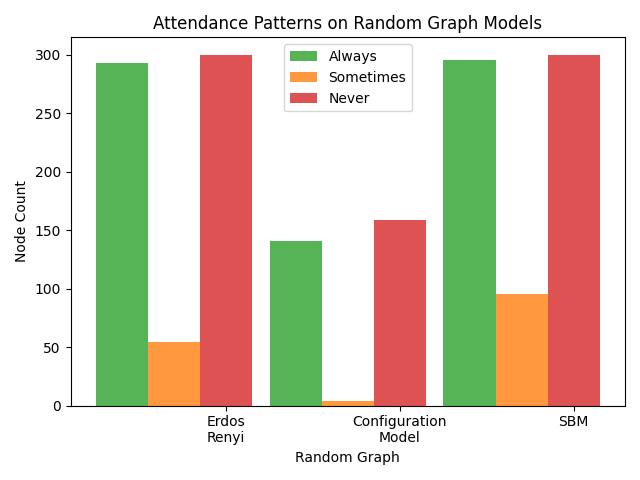
\includegraphics[scale=0.7]{always_sometimes_never.png}
\end{center}
The 0 solution appears unstable.  Are these networks attaining the MFP?  Not if there are sometimes nodes.

Description of telephone tag.

\section{Analysis of Stability on Highly Structured Networks}

Unstabiliity of ring network and Von Neumann network.  Adding redundant edges adds stability.  Universal telephone tag.

\section{Noise?}
Adding noise allows encourages the telephone tag scenario to synchronize but also allows stable fixed points to erode?  Locally treelike networks with heterogeneous degree distributions may settle into something close to the maximal fixed point.  Punctuated equilibria on SBM.

\section{Discussion and Future Work}
Heterogeneity of network topology vs. heterogeneity of strategy.

Future: Analyze composition and stability of fixed points in random graph models.  Apply to real social networks.

\section*{Code}

\end{document}